\chapter{Sequence alignment}

\label{kap:sequence_alignment} % id kapitoly pre prikaz ref

In bioinformatics, a sequence alignment is a way of arranging the sequences of DNA, RNA, or protein
to identify regions of similarity that may be a consequence of functional, structural, or
evolutionary relationships between the sequences. \cite{Gollery2005BioinformaticsSA}

\section{DTW - dynamic time warping}
Dynamic time warping (DTW) finds similarity between sequences. It is one of the similarity methods
used in pattern recognition and time series data mining and other fields. Figure 1 shows example
of non-warping and warping between time series. DTW is efficient similarity method for time series
datasets, but it has quadratic complexity.

\begin{figure}[H]
  \centerline{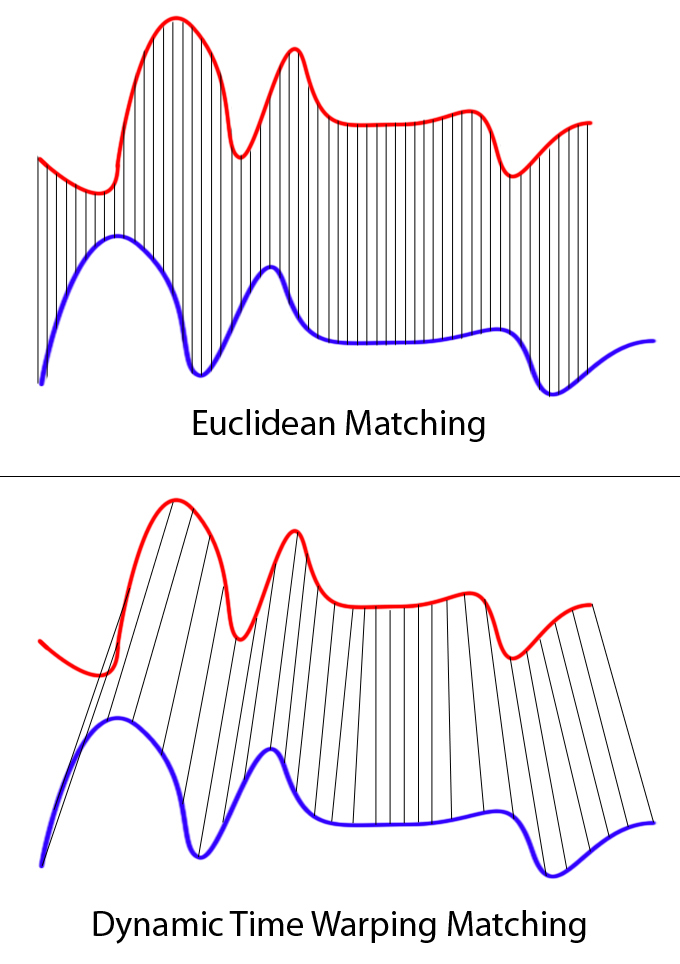
\includegraphics[width=0.4\textwidth]{images/dtw}}
  \caption[DTW]{DTW visualization}
  \label{obr:minion}
\end{figure}

TODO: how it works

\section{Needleman-Wunsch algorithm}

\section{FastDTW algorithm}

\section{Efficient DTW Algorithm}
